\documentclass[a4paper,11pt]{report}
%
%--------------------   start of the 'preamble'
%
\usepackage{graphicx,amssymb,amstext,amsmath}
\usepackage[includeheadfoot]{geometry}
\usepackage{fancyhdr}
\usepackage{indentfirst}
\usepackage{hyperref}

\geometry{ hmargin=2.3cm, vmargin=1.3cm }
%
%\usepackage{a4wide}
%
%\usepackage{geometry}
%%    homebrew commands -- to save typing
\newcommand\etc{\textsl{etc}}
\newcommand\eg{\textsl{eg.}\ }
\newcommand\etal{\textsl{et al.}}
\newcommand\Quote[1]{\lq\textsl{#1}\rq}
\newcommand\fr[2]{{\textstyle\frac{#1}{#2}}}
\newcommand\miktex{\textsl{MikTeX}}
\newcommand\comp{\textsl{The Companion}}
\newcommand\nss{\textsl{Not so Short}}

%
\hypersetup{
     backref=true,
     pagebackref=true,
     hyperindex=true,
     colorlinks=false,
     breaklinks=true,
     citecolor=black,
     filecolor=black,
     linkcolor=black,
     linkbordercolor= {1 1 1},
     citebordercolor= {1 1 1},
     bookmarks=true,
     pdftitle={Training Period Report - Surgical Planning Laboratory},
     pdfauthor={Nicolas Rannou},
     %&pdfsubject={NIMS: Neurobiological Imaging Management System},
     %pdfkeywords={data sharing, database, neurobiological images, open-source, metadata, workflow, ontology}        
}

%---------------------   end of the 'preamble'
%
\begin{document}
%-----------------------------------------------------------

\pagestyle{fancy}
\fancyhead{}
\fancyfoot{}

\fancyfoot[L]{Nicolas RANNOU}
%\fancyfoot[C]{DO NOT COPY OR DISTRIBUTE}
\fancyfoot[R]{Page \thepage}
%\fancyhead[C]{CONFIDENTIAL}
\fancyhead[L]{Training Period Report}
\fancyhead[R]{Surgical Planning Laboratory}
\renewcommand{\headrulewidth}{0.3pt}
\renewcommand{\footrulewidth}{0.3pt}

%Redéfinition du style fancy - plain, utilisé pour les pages de nouveau chapitre
%Le style par défaut est un style plain
\fancypagestyle{plain}{
\fancyhf{}
\renewcommand{\headrulewidth}{0.3pt}
\renewcommand{\footrulewidth}{0.3pt}

 %Définition des headers identiques à une page normale
\fancyfoot[L]{Nicolas RANNOU}
%\fancyfoot[C]{DO NOT COPY OR DISTRIBUTE}
\fancyfoot[R]{Page \thepage}
%\fancyhead[C]{CONFIDENTIAL}
\fancyhead[L]{Training Period Report}
\fancyhead[R]{Surgical Planning Laboratory}
}


\begin{titlepage}

%\addtolength{\topmargin}{-3cm}
%\addtolength{\textheight}{28cm}
%\setlength{\textwidth}{19cm}
%\setlength{\oddsidemargin}{-1cm}
%\setlength{\footskip}{-3cm}
%\addtolength{\textheight}{2cm}
%\addtolength{\hoffset}{-1cm}
%\addtolength{\textwidth}{2cm} 
%\enlargethispage{2cm}
\begin{center}
%\vspace{4in}

\begin{center}
\begin{minipage}[c]{.45\textwidth}\centering

\includegraphics[width=1\textwidth]{Images/Logos/logo_ISEN.jpg}
\begin{small}\textbf{Institut Supérieur de l'Electronique et du Numérique}\\Tel. : +33 (0)2.98.03.84.00\\Fax : +33 (0)2.98.03.84.10\\CS 42807 - 29228 BREST Cedex 2 - FRANCE\end{small}
\end{minipage}
\hfill\begin{minipage}[c]{0.3\textwidth} 
\begin{center}\textbf{
\begin{Huge}N5\end{Huge}
\begin{normalsize}\\School Year 2008/2009\\Training Period\end{normalsize}}
\end{center}

\end{minipage}
\end{center}

\bigskip
\bigskip
\bigskip

\hrule
\bigskip
\begin{minipage}{1\textwidth}
\begin{center}\begin{LARGE} Parameter space exploration and tools for fast visualization in EM segmentation and MRI bias field correction in Slicer 3
\end{LARGE}\end{center}
\end{minipage}
\bigskip
\hrule

\bigskip
\bigskip
\bigskip

\begin{small}From April 6th to August 31th \\ 
At \\ 
Surgical Planning Laboratory (SPL)
\end{small}


\includegraphics[width=.3\textwidth]{Images/Logos/logo_spl.jpg}
\begin{small}\\Brigham \& Women's Hospital\\
 Harvard Medical School \\
 75 Francis St. \\
 Boston, MA 02115\end{small}
%\vskip 1in
\end{center}
\vspace{0.5cm}
\begin{tabular}{*{2}ll}
\underline{Supervisors:} &Ron KIKINIS - SPL, Harvard Medical School - kikinis@bwh.harvard.edu\\
&Sylvain JAUME - CSAIL, Massachusset's Insitut of Technologies - sylvain@csail.mit.edu\\
\end{tabular}
\vspace{0.5cm}\\
%referring tearchers
\begin{tabular}{*{2}l}
\underline{Referring Tearchers:} &Christine CAVARO-MENARD - M2 SIBM - christine.menard@univ-angers.fr\\
&Dominique MARATRAY - ISEN Brest - dominique.maratray@isen.fr
\end{tabular}
\vspace{0.5cm}\\
%Etudiant
\begin{flushright}by Nicolas RANNOU\end{flushright}

\end{titlepage}
%-----------------------------------------------------------
\begin{abstract}
A couple of sentences on three or four lines to summarise your work.\\ 
This is a \LaTeX\ template for undergraduate project reports.\\
Its detailed contents evolve to reflect FAQs.\\
Expectation-maximization is very popular for segmentation but it can be tricky to understand and to use.
A full description of the EMS algorithm is done in this report.
Different methods for fast parameters exploration are described.
As part of the research, preprocessing methods like MRI bias field correction will be explained.
The results obtained will be presented.
Following the new workflow should allow the user to segment more datasets, more accurately.\\
%
\textbf{\underline{Keywords:}} segmentation, expectation, maximization, correction, bias.\\

\bigskip

\begin{center}\textbf{ Resum\'e }\end{center}
Quelques phrases pour resumer mon travail.\\ 
C'est un template \LaTeX\ pour les rapport.\\
Le contenu peut evoluer.\\
%
\textbf{\underline{Mots cl\'es :}}segmentation, expectation, maximisation, correction, biais.
%

\bigskip

\end{abstract}

%-----------------------------------------------------------
\tableofcontents
\addcontentsline{toc}{chapter}{Contents}
\listoffigures
\addcontentsline{toc}{chapter}{List of figures}
%-----------------------------------------------------------
\chapter{Introduction}
%The first chapter of a well-structured report is always an
%introduction, setting the scene with motivation and context (as in
%Sec.~\ref{context}) and then looking ahead to summarise what's in the
%rest of the report (as in Sec.~\ref{intro:contents}). It's the
%bit that readers look at first --- {\em so make sure it hooks them!}
%
%\section{Presentation of the laboratory}\label{intro}
%%
%\subsection{Harvard Medical School}
%Harvard Medical School (HMS) is one of the graduate schools of Harvard University. It is currently ranked first among American medical schools by U.S. News and World Report.\\
%%
%\begin{figure}[!h] % Un peu plus impératif que le h
%\begin{center}
%
\includegraphics[width=0.3\textwidth, scale=0.25]{Harvard_shield_Medical.jpg}                                                                                    
%\end{center}
%\caption{Harvard Medical School's shield}
%\end{figure}
%%
%Located in the Longwood Medical Area of the Mission Hill neighborhood of Boston, Massachusetts, H.M.S. is home to more than 1200 students.\\
%The school has a large and distinguished faculty to support its missions of education, research, and clinical care. These faculty hold appointments in the basic science departments on the HMS Quadrangle, and in the clinical departments located in multiple Harvard-affiliated hospitals and institutions in Boston. There are approximately 2,900 full- and part-time voting faculty members consisting of assistant, associate, and full professors, and over 5,000 full or part-time non-voting instructors.
%%
%\subsection{The Brigham \& Women's Hospital}
%Recognized internationally for its excellence in patient care, its outstanding reputation in biomedical research, and its commitment to educating and training physicians, research scientists and other health care professionals, Brigham \& Women's Hospital (BWH) is a 777-bed teaching affiliate of Harvard Medical School located in the heart of Boston's renowned Longwood Medical Area. Along with its modern inpatient facilities, BWH boasts extensive outpatient services and clinics, neighborhood primary care health centers, state-of-the art diagnostic and treatment technologies and research laboratories.
%%
%\begin{figure}[!h] % Un peu plus impératif que le h
%\begin{center}
%
\includegraphics[width=0.3\textwidth, scale=0.25]{brigham_and_womens.jpg}                                                                                    
%\end{center}
%\caption{BWH's shield}
%\end{figure}
%%
%\subsection{The Surgical Planning Laboratory}
%The  Surgical Planning Laboratory (SPL) is a research laboratory in the Department of Radiology of Brigham and Women's Hospital. The Core Mission of the SPL is the extraction of medically relevant information from diagnostic imaging data and to concepts of computation and image analysis to new field of biomedical research. The lab collaborates with groups within Brigham and Women's Hospital, with other researchers at the Harvard Medical School, with local universities such as Harvard and MIT, and with clinicians, researchers, and engineers throughout the world.
%%
%\begin{figure}[!h] % Un peu plus impératif que le h
%\begin{center}
%
\includegraphics[width=0.3\textwidth, scale=0.25]{logo_spl.jpg}                                                                                    
%\end{center}
%\caption{SPL's shield}
%\end{figure}
%
\section{Context and motivation}\label{intro:context}
%My training...

Nowadays, medical image processing is becoming a major field of research in most of the laboratories. Indeed, because of the increasing complexity of the data they have to deal with,  physicists need something to help. Help must be provided in many different ways. Before the surgery, to etablish a fast and accurate diagnosis. During the surgery to prevent physicians from errors and to help them to proceed to more precise moves. After the surgery, to see if it succeeded, or to follow the pathology of a patient. The informations brought to the physicians by the tools must be accurate, robust and provide a fast feedback.
%
\par
%
In this context of pre and post operation, plenty of work has already been done. Nevertheless, there is still a lot of work to achieve. Regarding data storage and exchange, the increasing among of information leads us to find more approriate methods for the same purpose. Another interesting contribution of computer science to medicine is image segmentation. New methods have to be developped for a better diagnosis, or to detect new pathologies. A lot of segmentation techniques appeared like level-set segmentation, region growing or texture based segmentation. Each one is adapted to a specific problem like vessel segmentation or tumor detection. Another remarkable contribution is the segmentation based on expectation maximization (EM). It is very well suited for brain tissue segmentation. 
%
\par
%
For segmentation of brain MR images, the Surgical Planning Laboratory (SPL) at the Brigham and Women's Hospital, affiliated to Harvard Medical School, has developped an EM algorithm for segmentation. This model assumes that the MR volumes does not exhibit an intensity inhomogeinity. Moreover, the implementation is not widely used so far, because the complexity of the segmentation process. Finally, some steps seem not very accurate. In this report we will present an approach to enhance the segmentation for inhomogeneous MR images, correcting intensity bias field. We will also provide tools to the end-user for an easier and more accurate segmentation process.
%
%BUT -  So far, the expectation maximization segmentation (EMS) module not used by physicists.
%Indeed, the results are highly dependents on chosen parameters and some parameters estimation may be hard to do.
%Making something easy to use and one which one the user has more control appears to be an obligation.\\
%FINALLY - OR LATER - In this report, we will first introduce you to the EMS algorithms, especially the one implemented in Slicer 3.
%Then, the new tools available in this EMS workflow will be presented.
%Finally, the new results obtained with the new segmentation process will be evaluated through some experiments.
%
%
%This is a template for \LaTeX\ project reports in the Department of
%Mathematical Sciences. It shows a good overall structure for the
%printed document, and shows how to construct it with a master file
%(\texttt{report.tex}) plus subsidiary files (\texttt{chap1.tex},
%\dots, \texttt{app1.tex}, \dots, \texttt{biblio.tex}).
%\par
%At the same time, features of the current version of \LaTeX\ (\LaTeXe)
%are illustrated --- such as mathematical expressions, numbering and
%cross-referencing, bibliography and citations, graphics and tables.
%Comparison of the source files with the printer-ready document will
%answer a few FAQs: \Quote{How can I do \dots\ in \LaTeX?}.
%\par
%However, this is {\em not} a textbook on \LaTeX\ --- for that, use the
%\lq\nss\rq\ notes by Oetiker \etal\ \cite{NSS}. They are written for
%novices, and are a pleasure to read. They are available free on-line,
%and are kept up-to-date. The \LaTeX\ book at \textsl{Wikipedia}
%\cite{WL} includes the \nss\ material and is good for reference too.
%Access these via the \LaTeX\ resources page \cite{LAT}.
%\par
%For more advanced features see \eg\lq\comp\rq\ \cite{MG}.
%\par
%Well-meant advice on \LaTeX\ for report-writing and poster-making is
%available\footnote{From  \texttt{bob.johnson@dur.ac.uk}} in room CM315,
%where there are reference copies of both \comp\ \cite{MG} and
%\textsl{The Graphics Companion} \cite{GRM}.
%\par
%Even if you are misguided enough \cite{AC} to prepare your report in
%\textsl{Word}, this template at least exemplifies a good structure ---
%and gives advice about references and help with typography.

%
\section{Contents}\label{intro:contents}
The main body of this report is divided as follows.
\par
Chapter \ref{sec:EM} focuses on the EM segmentation. Background will be reminded and the algorithm used in the SPL will be fully described. We will also present in this chapter the segmentation workflow developped in the SPL and the limitations of the current implementation.
Chapter \ref{sec:contributions} describes our contributions. It explains the solutions brought to enhance the segmentation and to improve the usability of the current framework.
Chapter\ref{sec:results} shows the results obtained. It aslo discussed about the results obtained. An expert radiologist evaluates the segmentation. Finally, the work which still has to be done in order to enhance the segmention is briefly describe.
%
%The main body of this report is divided as follows.
%\par
%Chap.~\ref{sec:formulas} has some examples of mathematics, then
%Chap.~\ref{sec:graphics} deals with graphics and includes
%Sec.~\ref{sec:tables} about tables. The Conclusion, in
%Chap.~\ref{andfinally}, summarises what's been achieved, the open
%questions and what could be done next.
%\par
%Then comes the Bibliography, listing all sources of material, data and
%computer programs used, \etc. Its construction is explained in
%\cite[Sec.~4.2]{NSS} and there's more about it in App.~\ref{app:refs}.
%\par
%Otherwise appendices typically hold basic background theory, or
%additional or similar examples, or longer proofs (App.~\ref{app:proofs})
% --- anything you need but which would hold up the main flow of the
%story. You could also use an appendix for listings of any computer
%programs that you've written (App.~\ref{app:programs}).
%\par
%Here there's information about using a PC (App.~\ref{app:pc}) plus
%brief advice on grammar and typography (App.~\ref{app:typo}).

%-----------------------------------------------------------
%Background
\chapter{Background and similar projects}
\section{General background}
\par
Electronic data sharing has become an important tool in many scientific disciplines. This is especially true for those that work with large and complex data sets as. Thus, the value of data sharing has become increasingly apparent to scientists involved in neuroimaging for several reasons. The volume of data generated with brain imaging techniques is striking, and continues to be one of the most rapidly growing areas in this domain. Moreover, published findings reflect only a fraction of the data originally collected. The data themselves take a variety of forms and typically are not accessible for widespread sharing and use. Making neuroimaging data more accessible for sharing would facilitate the comparison of findings across laboratories.
\par
However, unlike fields in which databasing efforts have been successful, there are no universally accepted standards for the structure and content of neuroimaging data sets. Data formats vary widely across different laboratories and neuroimaging methods. This diversity of data and formats reflects several factors, including the rapid developments within the field and the rapid changes in our knowledge about brain. Indeed, neuroimaging methods are evolving quickly, and changes are sometimes accompanied by substantial changes in data content that directly affect  the format. For example, with the transition from anatomical to functional MRI, data formats changed from three to four dimensional. More critically, imaging of brain function demands a clear specification of the behavioral conditions under which the data were acquired. This is linked to the scientific hypotheses being tested. The number of potentially important behavioral variables is large and poorly defined.
\par
The figure 2.1 shows a part of the issues related to data sharing that need to be answered when researchers work on such projects.
\begin{figure}[!h]
\begin{center}
\includegraphics[scale=0.65]{images/database_issues.png}
\caption{\small Issues related to neuroimaging databases}
\end{center}
\end{figure}
\par
Faced to these issues and recognizing the increasing need for data sharing within the neuroimaging community, several groups have conducted researches to develop neuroimaging databases. Different models have been explored. Some use a centralized model that directly manages the storage and distribution of data. Others use a distribution model, in which a centralized listing is maintained that describes the available data and their location, whereas the data themselves are stored locally, under the control of their owner. The diversity of databases projects is a good thing to explore various approaches and to value each of them. In the next pages, we will review some of the most interesting projects conducted by team across the world, which proves the importance given to this research since several years. 

\section{The Human Imaging Database, by the BIRN}
\par
The Biomedical Informatics Research Network (BIRN) is a research American project launched in 2001 and supported by the National Institutes of Health's National Center for Research Resources (NCRR). It is one of the best known and complete work related to the sharing of data in the field of biomedical. It is composed by around 35 laboratories across the United States of America. The main goal of the projects is to propose a geographically distributed virtual community of shared resources associated with a large range of tools.
\par
As part of their huge work, the BIRN has been working on the Human Imaging Database (HID) which is an extensible database management system. It has been developed and implemented to address the problems associated with managing the increasingly large and diverse datasets collected as part of the morphometry and function BIRN (mBIRN, fBIRN) collaboratories. This system is comprised of three core components, among them, The Human Clinical and Imaging Database itself and an intuitive web based user interface.
\par
The database is composed of an extensible schema and structured core. The core database contains a hierarchical description of an experiment and how experimental protocols relate to this hierarchy. Then, the database at a particular site can be extended to contain relevant information concerning the research subjects used in an experiment, subjects assessments, the experimental data collected, the experimental protocols used and any annotation or statistics (metadata) normally included with an experiment. The database can be extended utilizing extended tuples which can be re-used and/or modified for other experiments. The complete system is used to manage and query local data at various research sites within BIRN. In addition to local operations, the system allows for mediated queries across multiple federated databases allowing researchers to discover data across all relevant sites. There are currently 12 federated HID databases, 11 Oracle and 1 PostgreSQL versions, storing clinical information.
\par
Regarding the user interface, the figure 2.2 shows his overall structure based on three tier Java 2 Enterprise Edition (J2EE) architecture. It consists of a client tier, a server/JSP based middle tier and a relational database based enterprise information source (EIS) tier. The EIS tier consists of the Human Clinical and Imaging Database and a collection of stored procedures/packages for low level data access functions. The middle tier currently consists of a web tier tier only. The underlying web application framework used for user interface is Jakarta Struts. It uses a controller servlet to intercept a web request and determine what to display next. The business logic layer is defined as the code manipulating business data (e.g. clinical assessments) relevant to the application. DAO is for Data Access Objects. Each software layer communicates with neighbor layers via well defined interfaces, which remain stable while the actual implementation can change drastically over time facilitating software maintenance and robustness.
\begin{figure}[!h]
\begin{center}
\includegraphics[scale=0.7]{images/birn.png}
\caption{\small Human Imaging Database Graphical User Interface structure\protect\footnotemark}
\end{center}
\end{figure}
\par
Thus, the projects conducted by the BIRN are very interesting in our case, especially the Human Imaging Database which provide a web-based interface and a relational database back-end for storing and managing brain imaging data. I will come back later on BIRN's works regarding the ontologies with NeuroLex (formerly BIRNLex).

\section{The Functional Magnetic Resonance Imaging Data Center}
\par
\footnotetext{Extracted from Ozyurt and al.,(2004) Web- accessible clinical data management within an extensible neuroimaging database. Society for Neuroscience, Washington, DC, 2005 Online}
The Functional Magnetic Resonance Imaging Data Center (fMRIDC) founded in 1999, has been thought to establish a facility for the sharing of functional neuroimaging data within the community of neuroscience. The Data Center has received during several years study data from fMRI analyses published in the Journal of Cognitive Neuroscience. Researchers exchange data with the Data Center through two simple means: contributing study data to the archive, in which researchers fill out detailed forms describing study protocols and individual subject information, and requesting study data from the record of studies in the repository.
\par
To address the problems associated with managing the increasingly large and diverse datasets collected, an object-relational database schema called Neurocore was developed. By exploiting the object-oriented properties of object-relational database technologies, Neurocore is a database architecture that is completely modifiable while maintaining a standard core structure.  Thus, this methodology can be used to extend the database to contain relevant information concerning the research subjects used in an experiment, the experimental data collected, the experimental protocols used and any annotations or statistics normally included with an experiment. The core database contains a hierarchical description of the experiment and how experimental protocols relate to this hierarchy. The ability to extend experimental descriptions in the database is accomplished through the use of object-relational technologies. This is very similar as the previous project (BIRN) exposed above.
\begin{figure}[!h]
\begin{center}
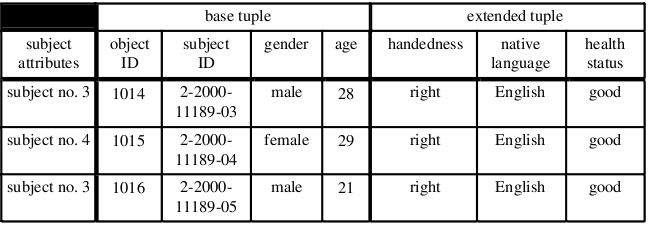
\includegraphics[scale=0.8]{images/fMRIDC_descriptor.png}
\caption{\small Descriptor ``subject'' in the database\protect\footnotemark}
\end{center}
\end{figure}
\footnotetext{Extracted from Van Horn, J.D., et al., The Functional Magnetic Resonance Imaging Data Center (fMRIDC): the challenges and rewards of large-scale databasing of neuroimaging studies, Science 356 (2001), 1323-1339}
\par
As shown in the figure 2.3, the inherent attributes for an entity constitute the ``base tuple'' that defines the minimum informational requirements for that entity. These base tuples can then be extended with additional attributes through the definition of an extended tuple. Furthermore, the extended tuples can be reused and/or modified for other experiments, and be used to guide future interactive data entry forms.
\par
Regarding the physical architecture of the fMRIDC computional resource, it is implemented in three tiers: the client Web browser (using HTML, XML, Java and Javascript), the web server running PHP and Python software and the database management system itself.
\begin{figure}[!h]
\begin{center}
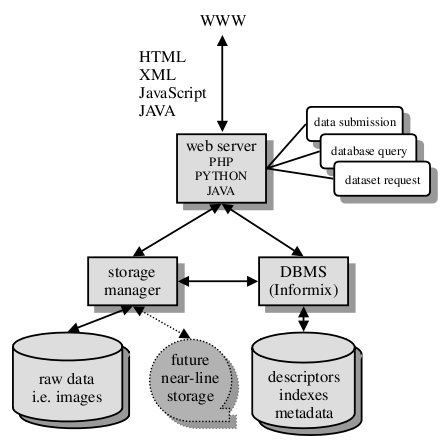
\includegraphics[scale=0.7]{images/fMRIDC_architecture.png}
\caption{\small Physical architecture of the fMRIDC\protect\footnotemark}
\end{center}
\end{figure}
\footnotetext{Extracted from Van Horn, J.D., et al., The Functional Magnetic Resonance Imaging Data Center (fMRIDC): the challenges and rewards of large-scale databasing of neuroimaging studies, Science 356 (2001), 1323-1339}
\par
Even if this project is relatively old compared to others presented here, it still remains very interesting by giving a specific structure for the overall system and by having specifics goals. Indeed, one of their main goal is to allow small and/or limited funded laboratories to access to a large bank of data in order to be able to reliably reproduced the fMRI results. Of course, they have implemented a very specific workflow to add data in the system in order to respect the human subject as well as the rights of the original authors. Unfortunately, the fMRIDC doesn't accept any new datasets but the others datasets can still be found on their website.
\section{The Computional Neuroscience Applications Research Infrastructure}
\section{The Extensible Neuroimaging Archive Toolkit}
\section{A work about other projects}







\chapter{The contributions}\label{sec:contributions}
In this chapter we will present all the contribution to enhance the segmentation workflow in Slicer 3. We propose solution to the problem cited in the previous chapter (\ref{su:limitations}). We get started with the registration problem. The we propose solutions to enhance the class selection and to allow the user to evaluate his selection. Finally, we present some tools we added to help the user to find the good intensity normalization value and an estimation of the global prior weights.
%
\section{MRI Bias Field correction}

The registration step could present some problems if the image to segment has intensities inhomogeinities. We remind the problem, then we present the solution proposed.

\subsection{Interest}

In the segmentation process, a registration step is required. Registration consists in finding a trasformation to fit two images as well as possible. It is described in details in DSFSDF. Only one pre-processing (intensity normalization) is done before the registration. The problem is that the algorithm is designed to treat MR images. MR images are often corrupted by a bias field. Thus, the the image to register presents intensities inhomogeinities. These inhomogeinities can deteriore a lot the registration.
\par
On figure (\ref{fig:bfexemple}), we present the result of the registration between an atlas and a biased MR image. Note that the target MR image has been normalized to have the same mean value as the atlas. The results is clearly bad. A solution must be brought to enhance this step and so the segmentation.

  \begin{figure}[ht]\centering
  \includegraphics[width=0.8\textwidth]{Images/Screenshots/badRegistration.png}
  \caption{Result of registration of a biased MR image without correction}\label{fig:bfexemple}
  \end{figure}
  
\subsection{Our approach}

The idea simply consists in correcting the bias field of the MR image before this step. Thus, the registration will be significantly enhanced.Since the registration is better, it should also increase the segmentation.
\par
To correct the bias field, we used the non-parametric approach presented by Styner in SDFSDF. We choose a non-parametric approach because it doesn't require prior information like the number of tissue to correct or the mean value of each tissue to correct. We implement an ITK\footnote{open-source C++ toolkit for segmentation and registration. See \cite{13}.} filter (\cite{14}) in Slicer 3. 
\par
We choose not to implement it in Slicer 3 as part as the EM Segment module. Indeed, users may want to correct the bias field in MR images for other purposes. Moreover, because it would be the first pre-processing step, it is possible to do so. The user will first have to correct the intensities inhomogeinities via the module then use the corrected images in the EM segmentation module.
\par
We can describe the new segmentation workflow in Slicer 3 as we do in figure (\ref{fig:wfwbc}).



\begin{figure}[ht]\centering
  \includegraphics[width=1\textwidth]{Images/Graphics/bfnwf.png}
  \caption{New algorithm pipeline}\label{fig:wfwbc}
  \end{figure}
  
%\subsection{Results}
%corrected not corrected
%parameters explanation

%

\section{Class Distribution selection}\label{sec:CDS}
%
During parameters initialization, the user has to define each class distribution. The previous method of selection presented some limitations and we proposed a new approach.
%
\subsection{Interest}
%
So far, the user had two choices to define each class distribution. 
\par
The first possiblity consisted in entering manually the intensities mean value and variance for each class, for each volume to be processed. This way, the user can be very precise and accurate when he defines each class. But it is very hard to find the good mean value and variance for each class for each volume. Morever, each time we want to process a new volume, we have to redefine mean values and variances. It is not convenient and it can a lot of time to find accurate values for the parameter initialization. 
\par
The next approch consisted in defining a class model by manual sampling. For each class, the user clics in the related part of the volume. The problem with this method is that you compute your mean value and variance using only a few samples. Your sample will never be bigger that one hundred points because it is not convenient. Then, your mean values and variances are not accurate. Moreover, results are not reproducible with this method. This the number of samples is reduced, means and variances can vary a lot with one more sample and you can never reproduce two times the same initialization.
\par
Because of all these limitations,  we proposed a new approach using a label map, to estimate each class model.
%
\subsection{Method used}
%
The idea is to create a label map. This map contains colors. There is one color for each class we want to segment. The relation color/class is stored in $H$ (section ), in the EM algorithm. This relation color/class is set up during the tree creation step DSFSDF.
\par
The user creates a label map by coloring caracterisc regions for each tissue to segment, in the appropriate color. This gives a spatial information to the algorithm. It can now estimate automaticly the mean value and covariance of each class, for each tissue, using this label map.

\begin{figure}\centering
  \includegraphics[width=1\textwidth]{Images/Screenshots/labelmaps.png}
  \caption{Axial view of the label map.}\label{fig:labelmaps}
\end{figure}

\par 
It is very convenient because, since the algorithm needs a good initialization, we can easily define a sample of hundred of points for each class. The results will representatives. Moreover, the results are now reproducible. Indeed, we can store then re-use the same label map. The results will remain the same.

%
\section{Class Distribution visualization}\label{sec:tables}

An important contribution is a tool which allows to visualize the distribution of the classes to be segmented.
\subsection{Interest}
As discussed before, the algorithm is sensible to the initalization. It means that the initialization has to be good. Once the parameters are chosen, the user has no tools to know if his selection is accurate. Two classes to segment can't have too close means and variances. Even if the user sees the values he chooses, it is not easy to know if two classes to be segmented are too similar or not.
\subsection{Our approach}
The objective is to provide the user the most accurate and usefull vizualisation as possible.
\par
We first assumed that each class has a normal distribution. We first decided to plot the gaussian in 3D, using the multivariate normal distribution.
In the 2-dimensional nonsingular case, the probability density function is 
\begin{equation*}
f(x,y)=\frac{1}{2 \pi \sigma_y \sigma_y \sqrt{1-\rho^2}} \operatorname*{exp}\Big ( -\frac{1}{2(1-\rho^2)}\Big( \frac{(x-\mu_x)^2}{\sigma_x^2} + \frac{(y-\mu_y)^2}{\sigma_y^2} - \frac{2\rho(x-\mu_x)(y-\mu_y)}{\sigma_x \sigma_y}\Big)\Big)   
\end{equation*}
(see \cite{15}). $x$ and $y$ are the position of the pixel in the 2D space. $f(x,y)$ will return the value (heigth) of the $(x,y)$ pixel. Each $X$ and  $Y$ axe represent one volume. Let's first say that the range of the $X$ and $Y$ axes are the intensity range of the $X$ and $Y$ volumes. $\mu_x$ is the mean value of the class in the $X$ volume. $\mu_y$ is the mean value of the class in the $Y$ volume. $\sigma_x$ and  $\sigma_y$ are the variance of the tissue in its respective volume. $\rho$ is the correlation between $X$ and $Y$. It indicates the strength and direction of a linear relationship between two random variables ( see \cite{16}). 
\par
We can easily deduce $\rho$ from the covariance matrix $\Sigma$ (see \cite{17}). Indeed, in the 2D case, the covariance matrix can be expressed as

\begin{equation*}
\mathbf{\Sigma} = 
 \begin{bmatrix}
   \sigma_x^2 & \rho \sigma_x \sigma_y \\
   \rho \sigma_x \sigma_y & \sigma_y^2
 \end{bmatrix}
\end{equation*}


\section{Intensity Normalization}
\subsection{Interest}
usefull if you need to do a lot of segmentations
enhance the rescaling..?
\subsection{Our approach}
background/brain
%


\section{Global Prior Estimation}

The last contribution to the EMS is a tool which provides the user an easy and fast way to estimate the global prior weights (GPW).(ref ch2 ...)

\subsection{Presentation of the problem}
This contribution is usefull in many different ways.
When you run the segmentation process,at the 6th step of the process, you have to provide to the algorithm an estimation of the GPW for each node in the tree. 
First of all if there are a lot of structures to segment, they user can spend a lot of time during this step. Indeed, for each part of this tree strcuture, they have to define the GPW. Moreover, the user may not know at all which weights to choose. This new approach will provide the users a good estimations of the weights to use. We must also keep in mind that the end users are physicists. They might don't understand what the parameters meanings and providing them a visual feedback could help them a lot.
\subsection{Our approach}
We divided the problem in two parts. The first part will be about providing the user a real-time feedback regarding the GPW estimation.
The second part will consist in developping an algorithm which fills automatically the tree.
\subsubsection{Fast user feedback}
We can divide the feedback part in 3 steps: the histogram computation and utilisation, the multicolumn list and the labelmap generated.
The histogram allows the user to manual segment classes based on intensity.
The multicolumn list allows the user to change the order of the classes in the histogram.
The labelmap provides to the user a visual feedback, base on the segmentation realized in the histogram.
Using these three complementary tools, the user, even if he is not initiated can estimate easily, accurately and rapidely the GWP.
\\schema
\subsubsection{Global priors evaluation}
The algorithm used to estimate the weight of each node is iterative. It starts from the root and goes to the leaves. It evaluates the weight of the childs of the active node at each iteration. Here is a description of the algorithms used to compute the GPW of each node.\\
DEscirption algo 1\\\\
%
%
\begin{minipage}{1\textwidth}
%
\hrule
\textbf{\\Algorithm 1:} \textsc{TreeWeightEstimation}(R, W)
\hrule
%variables definition
\textbf{\\define}  C = CHILD(R) $\leftarrow$ set of childrens of root R\\ 
\textbf{define}  LEAF(C)      $\leftarrow$ set of leaves of tree with roots C\\ 
\textbf{define}  H            $\leftarrow$ set of structure-specific information defined by LEAF(C) for each leaf\\
%
\textbf{update} W in childrens of root R with the results of \textsc{WeightEstimation}(C,LEAF(C),H)\\
%
\textbf{for each} node R' in CHILD(R) that is not a leaf\\
%
$\triangleright$\textsc{TreeWeightEstimation}(R', W)\\
\hrule
%
\end{minipage}
%
\\\\\\Descripton algo2\\
The algorithm used estimates the global prior of the leaves of the current node, based on the number of pixel which belong to the child classes.
This number of pixels is calculated from the segmentation computed in the histogram.(CF ..)\\\\
%
\begin{minipage}{1\textwidth}
%
\hrule
\textbf{\\Algorithm 2:} \textsc{WeightEstimation}(C,LEAF(C), W,H)
\hrule
%variables definition
\textbf{\\define}  T $\leftarrow$ set of total weight of leaves in LEAF(C). Leaves weights are contained in H\\ 
\textbf{define}  E      $\leftarrow$ set of weight for each node of C\\ 
\textbf{for each}  node of C\\
$\triangleright$E=E+H : Get the total weight of each node\\
%
W=E/T\\
%
\textbf{return} (W)\\
\hrule
%
\end{minipage}
%


\chapter{Results and discussion}\label{sec:results}
This chapter will review what has been done and
mentions the main open questions.
\par
Results using different tools
\par
limitations
\par
improvement (in relation to limitations)
%
\section{Results}
%
Tests has been performed to show the utility of the work done. The results are presented below. The testings are comparaisons between the results obtained with the previous workflow and the new one. The results obtained will then be reviewed by a specialist to evaluate the previous and the new segmented datasets.
%
\subsection{Bias correction}
%
Here we get going with the intensities inhomogeinities correction.
%
\subsubsection{Testing process}
%
we create a mask.
%
\begin{figure}\centering
\includegraphics[width=1\textwidth]{Images/Screenshots/BiasCorrection.png}
  \caption{Module created for the bias correction.% On the left panel, there are the parametersto set for the correction. On the top left red box, the 2d mask is displayed. On the top right box, the 3d mask is shown. On the lower left yellow slice, the biased volume is presented. In the lower right slice, the corrected volume is printed
  }\label{fig:BiasCorrection}
\end{figure}

%
\subsubsection{Results}
%
Here are the resultsfdd ddddddddddd dddddddddddd ddddddddddd ddddddddd dddddddddd ddddddddddd dddddddddd dddddddddd ddddddddd dddddddddd ddddddddd dddddddd dddddddd dddddd dddd dddddddd..
%
\par
\begin{figure}\centering
\begin{minipage}[c]{.45\textwidth}\centering
  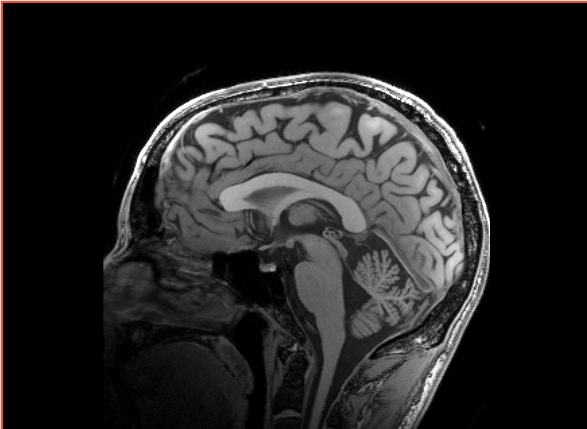
\includegraphics[width=.95\textwidth]{Images/Screenshots/T1SagittalNotCorrected.png}
  \caption{Sagittal view of a biased T1 volume.}\label{fig:T1SagittalNotCorrected}
\end{minipage}\hfill
\begin{minipage}[c]{.45\textwidth}\centering
  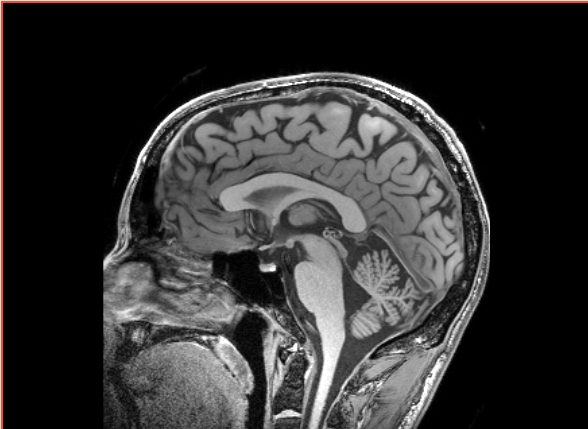
\includegraphics[width=.95\textwidth]{Images/Screenshots/T1SagittalCorrected.png}
  \caption{Sagittal view of the T1 volume after bias correction.}\label{fig:T1SagittalCorrected}
\end{minipage}
\end{figure}
%
\par
more comments ttttttttttttttttttttt ttttttttttttt ttttttttttt tttttttttttt ttttttttttt ttttttttttt tttttttttttttt ttttttttttttt tttttttttttttt tttttttttttt ttttttttttttttt\\
%
\subsubsection{Specialist's point of view}
%
\subsection{Global Prior estimation}
%
\subsubsection{Testing process}
%
\subsubsection{Results}
%
\subsubsection{Specialist's point of view}
%
\subsection{Class Selection}
%
\subsubsection{Testing process}
%
\subsubsection{Results}
%
\subsubsection{Specialist's point of view}
%
\section{Limitations}

\section{Future work}
\newpage
\section*{Acknowledgements}
\addcontentsline{toc}{chapter}{\numberline{}Acknowledgements}
Ron Kikinis who gave me the opportunity to carry out my intersnship in the SPL.
Sylvain Jaume who supervises me during all my work.
Andryi, Daniel, Steve?


%-----------------------------------------------------------
\addcontentsline{toc}{chapter}{\numberline{}Bibliography}
\begin{thebibliography}{9999}%\enlargethispage{\baselineskip}
%
\bibitem[1]{1}A.P. Dempster, N.M. Laird, and D.B. Rubin, "Maximum likelihood from incomplete data via the em algorithm", \textsl{Journal of the Royal Statistical Society: Series B}, vol. 39, pp. 1-38, November 1977.
%
\bibitem[2]{2}Y. Weiss, "Bayesian motion estimation and segmentation", \textsl{PhD thesis}, Massachussets Intitute of Technology, May 1998.
%
\bibitem[3]{3}R.C. Hardie, K.J. Barnard, and E.E. Armstrong, "Joint MAP registration and high-resolution image estimation using a sequence undersampled images", \textsl{IEEE Transaction on Image Processing}, vol. 6, pp. 1621-1633, December 1997.
%
\bibitem[4]{4}M. Murgasova, "Tutorial on Expectation-Maximization: Application to Segmentation of Brain MRI", May 2007.
%
\bibitem[5]{5}S. Borman, "The Expectation Maximization Algorithm",January 2009.
%
\bibitem[6]{6}Wikipedia, "Expectation-Maximization algorithm", \textsl{http://en.wiki.org/wiki/Expectation-maximization$\_$algorithm}, June 2009.
%
\bibitem[7]{7}G. McLachlan, and T. Krishnan, "The EM Algorithm and Extensions", \textsl{John Wiley \& Sons}, New York, 1996.
%
\bibitem[8]{8}K. V. Leemput, F. Maes, D. Vandermeulen et al., "Automated model-based tissue classification of MR images of the brain", \textsl{IEEE Transaction on Medical Imaging}, 18(10), pp. 857-908, 1999.
%
\bibitem[9]{9}K. V. Leemput, F. Maes, D. Vandermeulen et al., "Automated model-based bias field correction of MR images of the brain", \textsl{IEEE Transaction on Medical Imaging} 18(10), pp. 885-896, 1999.
%
\bibitem[10]{10}W. M. Wells III, W.E.L. Grimson, R. Kikinis et al., "Adaptative segmentation of MRI data", \textsl{IEEE Transaction on Medical Imaging} 15(4), pp. 429-442, 1996.
%
\bibitem[11]{11}K.M. Pohl et al., "A Hierarchical Algorithm for MR Brain Image Parcellation", \textsl{IEEE Transaction on Medical Imaging} 26(9), pp. 1201-1212, 2007.

%
\end{thebibliography}
%\vfill
%\begin{flushright}\small Prepared in \LaTeXe\ by RCJ\end{flushright}

%-----------------------------------------------------------
\appendix
%\chapter{About references}\label{app:refs}
Your report will be put together in your own style, mostly using your
own words. Much of it will be standard material that you've read and
digested, but you may have a fresh example, application or calculation
that you've done yourself.
\par
You must make clear what's not your own work by referring suitably
to your sources --- books or articles or web-pages, etc. Not to do so
can count as plagiarism, which is cheating.
\par
This appendix aims to amplify the advice given in the
Library's guide \cite{BR}, which you should read.
%----------------------------------------
\section{Organisation}
Follow the style of this template --- that is, put an orderly list of
your sources (\Quote{The Bibliography}) at the end of the main text,
and refer to (\Quote{cite}) items on the list by suitable codes placed
appropriately in the report's text.
\par
For your bibliography the golden rule is that each listed item must give
enough detail to allow readers to follow it up themselves and find the
precise part of the book, article, web-site or whatever without
ambiguity or delay.
\par
For instance it's no use saying just \Quote{The Times newspaper} unless
you also give the date and page, or just \Quote{Wikipedia} unless you
give the complete URL of the specific page, \dots\ and so on.
\par
It's always better to give slightly too much information --- e.g. you
might include the ISBN of a book too. A good level of information is
exemplified here and recommended in the Library guide \cite{BR}.
\par
If you need to cite different parts of e.g. a book for different things,
then list it (say AB) in the bibliography and give the different
citations as [AB,~page~32] and [AB,~Sec.~4.7] and so on. The \LaTeX\
\verb+\cite+ command allows for this (look it up!).
\par
Now you see why a bibliography list is better than lots of footnotes
--- it neatly allows such multiple citations. Too many footnotes make a
mess.
\begin{itemize}\item This bibliography uses short letter-code
keys in alphabetical order. It's one of several standard possibilities
\cite{BR} and is often preferred for economy and because the letter
codes\footnote{Note the punctuation of \lq letter-code' and \lq letter
codes' here.} can be chosen to be helpful mnemonics. Numerical codes,
for instance, can't.
\item Long lines (with URLs usually \cite{IM,PS}) may need to be split.
The \LaTeX\ hack used here to manage such line-breaks may not appeal to
everyone.\end{itemize}
%---------------------------------
\section{Doing it}
What things need a reference? The answer is --- anything you didn't work
out or invent yourself, but took from someone or somewhere else. You may
do that, so long as you say so \textit{and also make it clear you
understand it}. Don't copy blindly! Here are some
examples.\begin{itemize}
\item \Quote{the following explanation is taken from [LH]} --- if you've
copied word-for-word from the article by Laurel \& Hardy, which you
list as item LH in the bibliography. Direct quotation should be used
sparingly, and the text emphasised --- perhaps by use of the
\texttt{quotation} environment in \LaTeX.\par
Don't be tempted to copy from a book, or \texttt{ctrl-C/ctrl-V} from the
web, \textit{without} clearly admitting it. It's easy to detect, and
it's suicide.
\item \Quote{the following proof is in many textbooks, \eg
[LH,~page~16]} --- if it is, and you can't think of a different proof,
except perhaps for notation.
\item \Quote{the material in this section is based on Sec.~2.6 of [CL]
and Chap.~3 of [SH]} --- if you've combined into your own words the
account by Cagney \& Lacey with that by Starsky \& Hutch.
 \item \Quote{the following proof is adapted from Chap.~4 of [SJ]} ---
if (say) you've filled in the gaps in Smith \& Jones' proof, or perhaps
changed it from the case of general $n$ to your case $n=2$.
\item \Quote{these calculations were done with \textsl{Matlab} [MAT]
using the m-file listed in App.~\ref{app:programs}} --- where the
reference MAT is to the \textsl{MathWorks} website.
\item \Quote{these calculations were done with the TISEAN package [TIS]}
--- if you've downloaded this specialised package from a web-page whose
URL (and author's name, if available) is item TIS in the bibliography.
\item \Quote{the graph is taken from Morecambe \& Wise [MW, page 16]}
--- if you've scanned the figure from their book. Similarly, if you've
downloaded a \texttt{.jpg} file from a web-site, then give in the
bibliography the URL and author (if known). Such citations could go
either in the figure caption or in the associated text.
\item \Quote{the data are taken from [XY]} --- where XY gives the
source of the numbers you've analysed. This might be a journal or
an online databank, \etc. Generally the numbers themselves should be
left out
--- a summary table or a graph or two (plotted with \textsl{R} or
\textsl{Matlab} or \textsl{Maple}) is often enough. Occasionally raw
data might be supplied separately --- e.g. on a CDrom.
\end{itemize}
Often your supervisor or someone else gives you something --- such
as a set of data, or a useful \textsl{Maple} worksheet, or help with a
proof --- when the appropriate form of bibliography item is
\Quote{Dr~I~Newton, private communication, April 2007}. Similarly for
printed course material --- \Quote{Dr~I~Newton, lecture notes
for module MATH5033, Durham University, Epiphany Term 2007.}
\par
Generally, don't refer to things you haven't read. Textbooks may well
cite the Serbian-language journal where the result you want was
originally published. But you are not in the business of ascribing
credit for discovery. In \textit{your} report \textit{you} must cite the
book where \textit{you} actually got it from and not give any possibly
false impression that you fluently read technical Serbian.
\par
Likewise, you may want to quote from Euclid or Archimedes.
But cite the place where you found the English words with something like
\Quote{Archimedes said, \lq Eureka!\rq\ (as quoted by [AB])}.
\par
Summarising --- tell the truth (where you got it from), the whole truth
(give full details), and nothing but the truth (you don't read Serbian).
\par
Finally, if in doubt --- ask your supervisor.

\chapter{Statistics}\label{app:formulas} Here we present the main formulas we used in this reports and some fundamentals about probabilities.


\section{Fundamentals}\label{f:Fundamentals}

$P(A)$ is the probability that $A$ is realized.\\
\par
$P(A|B)$ is the probability that $A$ is realized, knowing $B$.\\
\par
$P(A,B)$ is the probability that $A$ and $B$ are realized at the same time.\\
\par
$P(A|B) = \frac{P(A,B)}{P(B)}$



\section{Bayes' theorem}\label{f:Bayes}
\subsection{Theorem}
Let $S$ be a sample of space. If $A_1,A_2,...A_n$ are mutually exclusive and exhaustive events such as $P(A_i)\neq 0$ for all $i$.Then for any event $A$ which is a subset of $S = A1\cup A_2 \cup ... \cup A_n$ and $P(A) > 0$ we have
\begin{equation*}
P(A_i|A)= \frac{P(A_i)P(A|A_i)}{\sum_{j=1}^n P(A_j)P(A|A_j)}
\end{equation*}

\subsection{Proof}
We have $S = A1\cup A_2 \cup ... \cup A_n$ and $A_i \cap A_j = \varnothing$ for $i \neq j$. Since $A \subseteq S$

\begin{align*}
\Rightarrow A &= A \cap S\\
              &= A \cap (A1\cup A_2 \cup ... \cup A_n)\\
              &= (A \cap A_1)\cup(A \cap A_2)\cup ... \cup(A \cap A_n)
\end{align*}
Moreover
\begin{equation*}
P(A \cap A_i) = P(A)P(A_i|A)
\end{equation*}

So

\begin{align*}
 P(A) &= P(A\cap A_1) + P(A\cap A_2) + ... + P(A\cap A_n)\\
      &= P(A)P(A_1|A) + P(A)P(A_2|A) + ... + P(A)P(A_n|A)
\end{align*}

And

\begin{equation*}
P(A|A_i) = \frac{P(A \cap A_i}{P(A)}
\end{equation*}

Finally we obtain
\begin{equation*}
P(A_i|A)= \frac{P(A_i)P(A|A_i)}{\sum_{j=1}^n P(A_j)P(A|A_j)}
\end{equation*}

\section{Jensen's inequality}\label{f:Jensen}
\subsection{Inequality}
Let $f$ be a convex function defined on an interval $I$. If $x_1,x_2,...,x_n \in I$ and $\lambda_1, \lambda_2, ... , \lambda_n \geq 0$ with $\sum_{i=1}^n \lambda_i = 1$,

  \begin{equation*}
  f(\sum_{i=1}^n \lambda_i x_i) \leq \sum_{i=1}^n \lambda_i f(x_i)
  \end{equation*}

\subsection{Proof}
To show that the theorem is true we proceed by induction.\\
\begin{itemize}
\item \textbf{Initialization}\\
This is trivial for $n=1$.\\
\item \textbf{Hypothesis at rank $n$} 

 \begin{equation*}
  f(\sum_{i=1}^n \lambda_i x_i \leq \sum_{i=1}^n \lambda_i f(x_i))\\
  \end{equation*}

\item \textbf{Demonstration at rank $n+1$}

 \begin{align*}
  f(\sum_{i=1}^{n+1} \lambda_i x_i ) &= f(\lambda_{n+1} x_{n+1} + \sum_{i=1}^n \lambda_i x_i)\\
                                     &= f(\lambda_{n+1} x_{n+1} + (1-\lambda_{n+1})\frac{1}{1-\lambda_{n+1}}\sum_{i=1}^n \lambda_i x_i)\\
                                     &\leq \lambda_{n+1} f(x_{n+1}) + (1-\lambda_{n+1})f(\frac{1}{1-\lambda_{n+1}}\sum_{i=1}^n \lambda_i x_i)\\
                                     &= \lambda_{n+1} f(x_{n+1}) + (1-\lambda_{n+1})f(\sum_{i=1}^n \frac{\lambda_i}{1-\lambda_{n+1}} x_i)\\
                                     &\leq \lambda_{n+1} f(x_{n+1}) + (1-\lambda_{n+1})\sum_{i=1}^n \frac{\lambda_i}{1-\lambda_{n+1}} f(x_i)\\
                                     &= \lambda_{n+1} f(x_{n+1}) + \sum_{i=1}^n \lambda_i f(x_i)\\
                                     &= \sum_{i=1}^{n+1} \lambda_i f(x_i)\\      
  \end{align*}
\end{itemize}

With a concave function (in opposition to convex), the inequality becomes:

 \begin{equation*}
  f(\sum_{i=1}^n \lambda_i x_i) \geq \sum_{i=1}^n \lambda_i f(x_i)
  \end{equation*}
%\chapter{Computer programs}\label{app:programs}
An Appendix is the place to list computer programs that you've
written, using the {\tt verbatim} environment \cite[Sec.~2.11.4]{NSS}.
\par
For example ---
\begin{verbatim}
    10 PRINT "HALLO SAILOR!"
    20 GO TO 10
\end{verbatim}

%\chapter{Using a PC}\label{app:pc}
You may want \LaTeX\ on your own computer.
\par
A popular version of \TeX/\LaTeX\ for a Windows PC is \Quote{MikTex}
\cite{MKT}. \miktex\ is free, and is available online for 
download \cite{LAT} or locally on a DVD from
\texttt{bob.johnson@dur.ac.uk}, room CM315. It's also installed on the
ITS Networked PC Service under \texttt{Programs | Miscellaneous}.
\par
To use \miktex\ easily you need a dedicated
editor or IDE\footnote{Computer scientists say \lq Integrated 
Development Environment'.}. A good one is \Quote{WinEdt} \cite{WDT}, 
which runs under all recent versions of Microsoft Windows and integrates 
well with \miktex. \textsl{WinEdt} is free for 31 days; to use
it thereafter costs about \$40.
\par 
Completely free rivals include \Quote{TeXnicCenter} \cite{TXC}, which is
provided on the \miktex\ DVD and also set up on the ITS Networked PC
Service under \texttt{Programs | Miscellaneous | MikTeX}.
\par
Others include \eg \Quote{WinShell} \cite{WSH}, but are untried.
\par
All these editors/IDEs have a familiar style of graphical user-interface
with a toolbar and pull-down menus for all the common tasks involved in
editing source files, running \LaTeX\ and viewing the results.

\chapter{Results of the segmentation}\label{app:results}
Here we present the results of segmentations in the case of manual and labelmap sampling. The left image represents the results of the segmentation after a manual sampling and the other image represents the results after a labelmap sampling.

%\section{Axial view}

  \begin{figure}[htb]\centering
  \includegraphics[width=1\textwidth]{Images/Screenshots/axialcomp.png}
  \caption{Axial view of the segmentation with different sampling methods}
  \end{figure}

%\section{Coronal view}

  \begin{figure}[htb]\centering
  \includegraphics[width=1\textwidth]{Images/Screenshots/coronalcomp.png}
  \caption{Coronal view of the segmentation with different sampling methods}
  \end{figure}

%\section{Sagittal view}

  \begin{figure}[htb]\centering
  \includegraphics[width=1\textwidth]{Images/Screenshots/sagittalcomp.png}
  \caption{Sagittal view of the segmentation with different sampling methods}\label{fig:NC_C_L}
  \end{figure}
%-----------------------------------------------------------
\end{document}
